% =============================================================================
% Section 9 — DNA Topology
% =============================================================================
\section{DNA Topology: Linking, Twist and Writhe}\label{sec:dnatop}

\begin{objectives}
\begin{itemize}[leftmargin=*,itemsep=1pt,topsep=1pt]
  \item State the Călugăreanu--White--Fuller theorem and identify which of its terms are topological.
  \item Prove that conserved linking forces an exact trade between twist and writhe.
  \item Explain why replication creates a topological problem that no amount of force can solve.
  \item Connect supercoiling to the polymerase fidelity of Sections~\ref{sec:proofreading}--\ref{sec:refutation}.
\end{itemize}
\end{objectives}

\subsection{Biological setting}

A replication fork unwinds the double helix at roughly $50$ base pairs per
second. Because the two strands are wound about each other, unwinding them
requires either rotating the entire chromosome ahead of the fork --- impossible
for a molecule of that length --- or storing the rotation as strain in the DNA
itself. The cell does the latter, then relieves the strain with topoisomerases.

The mathematics that describes this storage is not an analogy. It is a theorem
about closed ribbons, and the quantity it conserves is an integer.

\subsection{How the helix was established: reading Photo 51}\label{sub:photo51}

Before modelling the geometry we should ask how it is known, and the answer is a
diffraction pattern. A helix of radius $r$ and pitch $P$, illuminated along a
direction perpendicular to its axis, produces a transform given by the
Cochran--Crick--Vand theory: on the layer line indexed by $n$, at height
$Z = n/P$ in reciprocal space, the amplitude is
\begin{equation}\label{eq:ccv}
  F_n(R) \;\propto\; J_n\!\left(2\pi r R\right),
\end{equation}
with $J_n$ the Bessel function of the first kind. The maxima of successive $J_n$
move outward with $n$, and the locus of those maxima is the famous \emph{X}. Its
opening angle gives $P/r$ directly.

For a \emph{double} helix the two strands are offset along the axis by a fraction
$\delta$ of the pitch, and their contributions interfere:
\begin{equation}\label{eq:interf}
  I_n(R) \;\propto\; \left|J_n(2\pi r R)\right|^{2}\cdot 4\cos^{2}\!\left(\pi n \delta\right).
\end{equation}
Now take the B-DNA value $\delta = 3/8$, which is what the minor- and major-groove
widths amount to. At $n = 4$,
\[
  \cos\!\left(\pi \cdot 4 \cdot \tfrac{3}{8}\right) = \cos\!\left(\tfrac{3\pi}{2}\right) = 0,
\]
and the fourth layer line vanishes identically. A systematic absence of this kind
is not a weak feature to be argued over; it is a yes-or-no observation, and it is
present in Photo~51.

\begin{figure}[htbp]
  \centering
  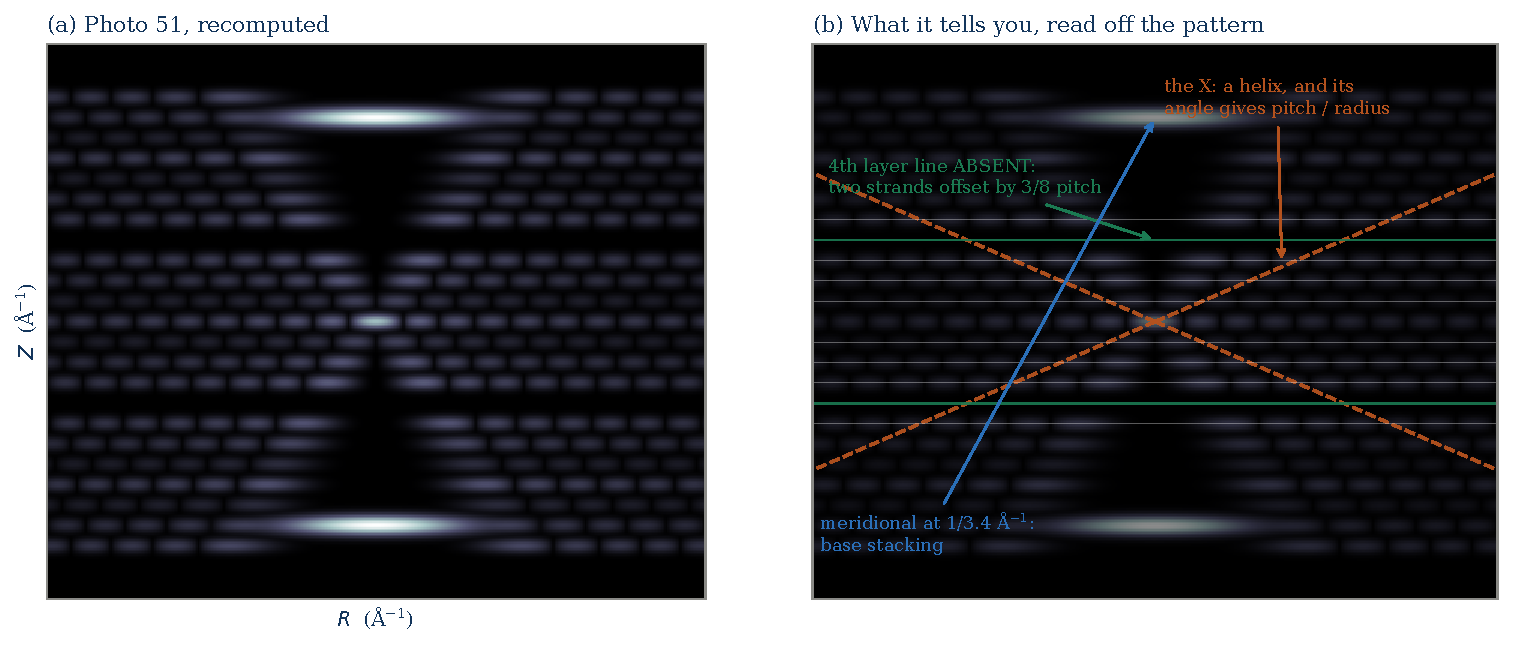
\includegraphics[width=\textwidth]{fig00_photo51.pdf}
  \caption{Photo~51, recomputed from \eqref{eq:ccv} and \eqref{eq:interf} with
  B-DNA parameters ($r = 10$\,\AA, $P = 34$\,\AA, rise $3.4$\,\AA,
  $\delta = 3/8$). This is not a traced copy of the plate: the features are
  outputs of the transform. (a) The pattern. (b) What it determines --- the helix
  cross fixing $P/r$, the meridional at $1/3.4\,\text{\AA}^{-1}$ from base
  stacking, and the fourth layer line (green) absent because
  $\cos(3\pi/2) = 0$. Generated by \file{scripts/textbook/make_figures.py}.}
  \label{fig:photo51}
\end{figure}

\begin{remark}[Why this belongs in a book about formal methods]
Equation~\eqref{eq:interf} is a derivation with no adjustable parameter at the
point that matters: given a two-strand helix with $\delta = 3/8$, the fourth
layer line \emph{must} be absent. This is the same logical shape as PSR$_2$ in
Section~\ref{sec:nogo} --- a parameter-free consequence, sharp enough that a
single observation decides it. Franklin's photograph was evidential precisely
because the structure it supported made a prediction that could have failed and
did not. The epistemics of 1952 and of this book are the same epistemics.
\end{remark}

\subsection{Mathematical development}

Model duplex DNA as a \emph{ribbon}: a closed space curve $C$ (the axis) together
with a unit normal field $u$ along it (pointing to one backbone). Three numbers
describe it.

\begin{definition}[Linking, twist, writhe]\label{def:lktwwr}
\begin{itemize}[leftmargin=*,itemsep=1pt,topsep=1pt]
  \item $\Lk$, the \textbf{linking number}, counts the signed crossings between
        the two edges of the ribbon. It is an \emph{integer} and a topological
        invariant: it cannot change under any deformation that does not cut a strand.
  \item $\Tw$, the \textbf{twist}, measures the rotation of $u$ about $C$,
        integrated along the curve. It is a real number and depends on geometry.
  \item $\Wr$, the \textbf{writhe}, measures the coiling of the axis $C$ in space,
        averaged over all viewing directions. It too is real and geometric.
\end{itemize}
\end{definition}

\begin{theorem}[Călugăreanu--White--Fuller]\label{thm:cwf}
For a closed ribbon, $\;\Lk = \Tw + \Wr$.
\end{theorem}

We do not prove this here --- it is a theorem of differential geometry, and the
proof would take the section far from biology. What we do prove is the
consequence that does the biological work.

\begin{theorem}[Twist--writhe trade-off]\label{thm:trade}
Suppose a segment is deformed between two states with the linking number
conserved, $\Lk_1 = \Lk_2 = \Lk$. Then
\[
  \Tw_2 - \Tw_1 \;=\; -\left(\Wr_2 - \Wr_1\right).
\]
Every turn of twist released by the helix reappears exactly as writhe of the axis.
\end{theorem}

\begin{proof}
By Theorem~\ref{thm:cwf}, $\Lk = \Tw_1 + \Wr_1$ and $\Lk = \Tw_2 + \Wr_2$.
Subtracting, $0 = (\Tw_2 - \Tw_1) + (\Wr_2 - \Wr_1)$.
\end{proof}

The content is in the \emph{exactness}. Strain is not dissipated by deforming the
molecule; it is only moved between two reservoirs. A cell cannot relax
supercoiling by wiggling. It must cut a strand --- which is what topoisomerases
do, and why they are essential genes and major drug targets.

\subsection{Formalisation}

In \file{formal/ANSE/GeneticsTextbook.lean}.

\begin{lstlisting}
theorem linking_conserved_twist_writhe (Lk Tw₁ Wr₁ Tw₂ Wr₂ : ℝ)
    (h₁ : Lk = Tw₁ + Wr₁) (h₂ : Lk = Tw₂ + Wr₂) :
    Tw₂ - Tw₁ = -(Wr₂ - Wr₁) := by linarith
\end{lstlisting}

The proof is one tactic, and it is worth being explicit about why so trivial a
formalisation is nevertheless worth having. What the Lean statement pins down is
the \emph{hypothesis structure}: the conclusion needs $\Lk$ to be the same number
in both equations, and nothing else. The companion
\lean{twist_writhe_needs_conservation} exhibits a pair of states where linking is
not conserved and the trade-off fails, confirming the hypothesis is load-bearing.
Formalising a triviality has no value; formalising which hypothesis a triviality
rests on sometimes does.

\begin{figure}[htbp]
  \centering
  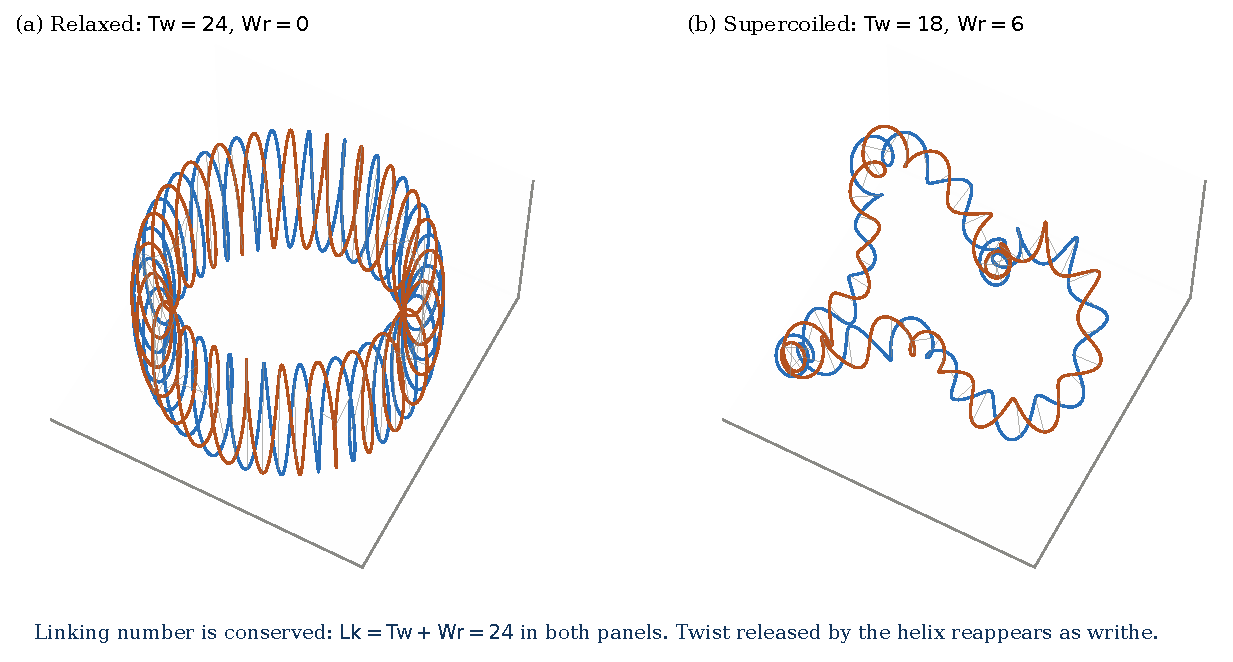
\includegraphics[width=\textwidth]{fig09_dna_topology.pdf}
  \caption{Two states of the same closed duplex at $\Lk = 24$. (a) Relaxed: all
  $24$ turns are twist, the axis is planar, $\Wr = 0$. (b) Supercoiled: six turns
  have been converted to writhe, the axis coils in space, $\Tw = 18$. The linking
  number --- the only topological quantity of the three --- is identical. Generated
  by \file{scripts/textbook/make_figures.py}, section~9.}
  \label{fig:supercoil}
\end{figure}

\subsection{Back to fidelity}

This section connects to the rest of the book through torque. A polymerase
elongating against accumulated positive supercoiling works against a mechanical
load, and the Bell--Kramers picture says a load modifies kinetic barriers
exponentially:
\begin{equation}\label{eq:bell}
  \gamma(\Gamma) \;=\; \gamma_0 \exp\!\left(\beta_{\mathrm{tor}}\Gamma\right).
\end{equation}
If torque raises the per-stage escape probability $\gamma$, then by
Proposition~\ref{prop:gain} the error rate rises geometrically in the number of
stages affected.

That is a hypothesis, not a result, and this book does not test it. It is
recorded here because it is the kind of coupling a student should notice: the
topological state of the template is a candidate input to the fidelity models of
Section~\ref{sec:proofreading}, and \eqref{eq:bell} would let it in through
$\gamma$ rather than through the repair capacity $c$ of Section~\ref{sec:mmr}.
Distinguishing those two routes experimentally would be a genuine contribution.

\begin{worked}[9.1: counting turns in a plasmid]
\textbf{Problem.} A relaxed circular plasmid of $3600$ bp has $\Lk_0 = 3600/10.5
\approx 343$ turns. A topoisomerase removes $17$ turns. If the resulting molecule
adopts a conformation with $\Wr = -14$, what is its twist, and what is the
superhelical density?

\textbf{Solution.} After the enzyme acts, $\Lk = 343 - 17 = 326$. By
Theorem~\ref{thm:cwf}, $\Tw = \Lk - \Wr = 326 - (-14) = 340$. The helix is
therefore still close to its relaxed twist of $343$, with most of the deficit
absorbed as negative writhe --- which is the usual outcome, because bending the
axis is energetically cheaper than over- or under-winding the helix.

The superhelical density is
$\sigma = (\Lk - \Lk_0)/\Lk_0 = -17/343 \approx -0.050$, close to the $\sigma
\approx -0.06$ typical of bacterial plasmids in vivo.
\end{worked}

\begin{exercise}
Using Theorem~\ref{thm:trade}, show that if a protein locally unwinds one turn of
helix ($\Delta\Tw = -1$) in a topologically closed domain, the compensating
writhe is exactly $+1$. Where does that writhe go physically?
\end{exercise}

\begin{exercise}
$\Lk$ is an integer; $\Tw$ and $\Wr$ are not. Explain how a sum of two
non-integers is forced to be an integer, and what breaks if the ribbon is not
closed.
\end{exercise}

\begin{exercise}
A replication fork advancing $1000$ bp introduces roughly $1000/10.5 \approx 95$
turns of positive supercoiling ahead of it. At $50$ bp/s, how many turns per
second must topoisomerase remove to keep the template relaxed?
\end{exercise}

\begin{exercise}[(harder)]
Using \eqref{eq:bell} and Proposition~\ref{prop:gain}, derive how the three-stage
error rate $\gamma(\Gamma)^3$ depends on torque, and state the measurement that
would test it. Why is it difficult to separate this from the repair-capacity
mechanism of Section~\ref{sec:mmr}?
\end{exercise}

\begin{ledger}
\textbf{Measured:} nothing in this section. The plasmid numbers in Worked
Example~9.1 are illustrative, chosen to match typical bacterial superhelical
densities; they are not a reported measurement. \\
\textbf{Assumed:} the ribbon model of duplex DNA, closure of the topological
domain, and --- for \eqref{eq:bell} --- a Bell--Kramers response of the kinetic
barrier to torque. The last is a hypothesis this book does not test. \\
\textbf{Proved:} Theorem~\ref{thm:trade} (\lean{linking_conserved_twist_writhe}),
with the control \lean{twist_writhe_needs_conservation}. Theorem~\ref{thm:cwf} is
cited, not proved, and is not formalised. \\
\textbf{Open:} whether template supercoiling contributes measurably to the
fidelity defects of Section~\ref{sec:refutation}, and whether that contribution
could be distinguished from a repair-capacity effect.
\end{ledger}
